\documentclass{article}
\usepackage[T1]{fontenc}
\usepackage{lmodern}
\usepackage{graphicx}
\usepackage{amsmath,amssymb}
\usepackage[a4paper,margin=2cm]{geometry}
\usepackage[absolute,overlay]{textpos}
\setlength{\TPHorizModule}{1mm}
\setlength{\TPVertModule}{1mm}
\usepackage[indonesian]{babel}
\usepackage{hyperref}
\setlength{\emergencystretch}{2em}
% unit: Halaman 7

\begin{document}

% === Halaman 7 (llm) ===

Hi rinaldi-m,

\vspace{20mm}

This message is sent on behalf of Benyamin Boy.
\small{Block future emails like this | Privacy policy}
\small{Zorpia Co. Ltd. P.O. Box \#28960, Gloucester Road Post Office, Hong Kong}

\vspace{10mm}

\centering{\textcolor{red}{\textbf{HATI-HATI! Jangan langsung klik jika anda tidak yakin!}}}

% deskripsi: Screenshot email phishing yang menunjukkan pesan palsu dari Benyamin dengan tombol 'Read Message' yang mencurigakan.
% bbox normalisasi: [0.1680, 0.1160, 0.8310, 0.6650]
\begin{textblock*}{139.23mm}(35.28mm,34.45mm)
\noindent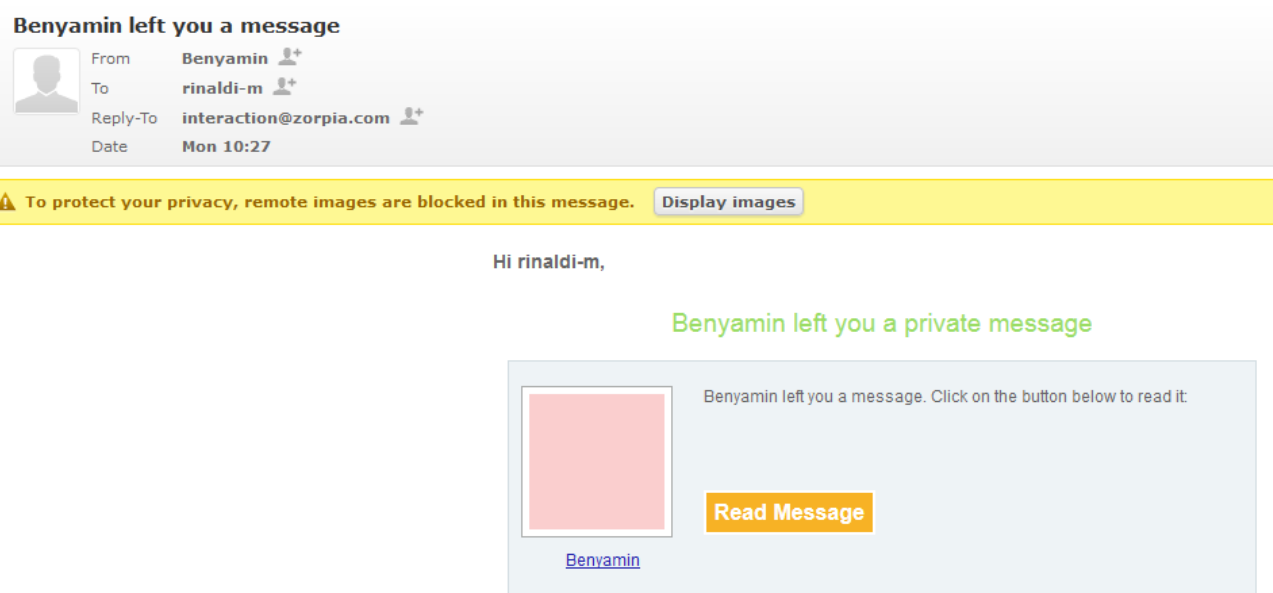
\includegraphics[width=139.23mm,height=163.05mm]{../../images/llm/page_007_img_01.png}%
\end{textblock*}

\end{document}
